
\vspace{-0.3\baselineskip}
\section{Dataset Preparation}
\vspace{-0.3\baselineskip}

\label{sec:data_collection}
\begin{table}[b]
\center
\vspace{-1\baselineskip}
\fontsize{7}{7}\selectfont
\hspace*{-0.1cm}
\setlength\tabcolsep{1.5pt}
\begin{tabular}{lcccc}
\toprule[0.13em]
% \thickhline
Dataset & Real data & Camera pose & 3D semantic map & Video per-pixel label   \\
\hline
\multicolumn{1}{l|}{CamVid~\cite{brostow2009semantic}}     &\checkmark        & -              & -              &  -   \\
\multicolumn{1}{l|}{KITTI~\cite{geiger2012we}}      &\checkmark  & \checkmark     & sparse points  & -   \\
\multicolumn{1}{l|}{CityScapes~\cite{Cordts2016Cityscapes}} &\checkmark  & -              &  -             & selected frames  \\
\multicolumn{1}{l|}{Toronto~\cite{wang2016torontocity}}    &\checkmark  & \checkmark     & 3d building $\&$ road & selected pixels \\
\hline
\multicolumn{1}{l|}{Synthia~\cite{RosCVPR16}}    & -          & \checkmark     & -       &\checkmark     \\
\multicolumn{1}{l|}{P.F.B.~\cite{richter2017playing}} &-   & \checkmark     & -     &\checkmark  \\
\hline
\multicolumn{1}{l|}{Ours}              & \checkmark &\checkmark    &dense point cloud  & \checkmark    \\
\toprule[0.13 em]
\vspace{-1.1\baselineskip}
\end{tabular}
\caption{Compare our dataset with the other related outdoor street-view datasets for our task. `Real data' means whether the data is collected from our physical world.
`3D semantic map' means whether it contains a 3D map of scenes with semantic label. `Video per-pixel label' means whether it has per-pixel semantic label.}
 %'Temporal variations' mean whether the recorded video can roughly cover the whole scene, but have multiple.
%\textcolor[rgb]{1.00,0.00,0.00}{we don't have temporal varations here, we didn't present results on this point neither, that last column needs to be removed. I would also argue the Toronto one is good.
%it has 3D model, so it is dense. In the scope of this paper, we want to paint the picture that 3D maps will be available, so we don't want to over-sell the  uniqueness of our data set.  }}
\label{tbl:data}
\vspace{-1.0\baselineskip}
\end{table}

\textbf{Motivation.}
As described in the \secref{sub:framework}, our system is design to work with available motion sensors and a semantic 3D map.
However, similar outdoor datasets such as KITTI and CityScapes do not contain such information, in particular the 3D map. The Tortoro City dataset~\cite{wang2016torontocity} that may be used is not open to public yet. As summarized in \tabref{tbl:data}, we list several key properties that are required to perform our experiments.
Note that none of existing public dataset satisfy our requirements.
% \textcolor[rgb]{1.00,0.00,0.00}{as I explained in the table, I suggest that we drop this argument, we need to have a 3D semantic map, none has it. the temporal effect needs to be tuned down, otherwise, it will be viewed as too narraow}
% for training, we want the recorded video to roughly cover the 3D environment, so that when new images come in, appearance similar views had been seen during training. This means repeated recording at similar spatial locations are required in the data, which we call temporal variations in \tabref{tbl:data}.
% However, most existing datasets are a temporal snapshot at some locations in the environment, which requires us to collect a new dataset ourselves.

\textbf{Data collection.}
We use a mobile LIDAR scanner from $Riegl$ to collect point clouds of the static 3D map with high granularity. As shown in \figref{fig:data}(a). The captured point cloud density is much higher than the Velodyne\footnote{http://www.velodynelidar.com/} used by KITTI~\cite{geiger2012we}.
% Amazingly, it is even able to capture the hight changes of curb on road.
Different from the sparse Velodyne LIDAR, our mobile scanner utilizes two laser beams to scan vertical circles. As the accquisition vehicle moves, it scans its surroundings as a push-broom camera. However, moving objects, such as vehicles and pedestrians, could be compressed, expanded, or completely missing in the captured point clouds.
In order to eliminate these inaccurate moving objects (circled in blue at \figref{fig:data}(b)), we conduct three steps:
1) scan the same road segment multiple rounds; 2) align and fuse those point clouds; 3) remove the points with low temporal consistency.
Formally, the condition to kept a point $\ve{x}$ in round $j$ is,
{\vspace{-0.5\baselineskip}
\begin{align}
\sum_{i=0}^{r}{\mathbbm{1}(\exists~\|\ve{x}_i - \ve{x}_j\| < \epsilon_d )} / r \geq \delta
\end{align}
}
where $\delta = 0.7$ and $\epsilon_d = 0.025$ in our experiments, and $\mathbbm{1}()$ is an indicator function. 
%Notice due to the symmetric property of $\ve{x}_i$ and $\ve{x}_j$, we obtain the static points for all rounds by looping over the points of a single round.
We keep the refined point clouds as a static background $\hua{M}$ for further labelling.

For video capturing, we use two frontal cameras with a resolution of \by{2048}{2432}. The whole system including the LIDAR scanner and cameras is well calibrated.
%\wrt the LIDAR scanner. Based on provided camera parameters from the hardware, all the images from videos are undistorted to match the 3D points.
% talk about registration and removing moving objects inside data

\begin{figure}[t]
\begin{center}
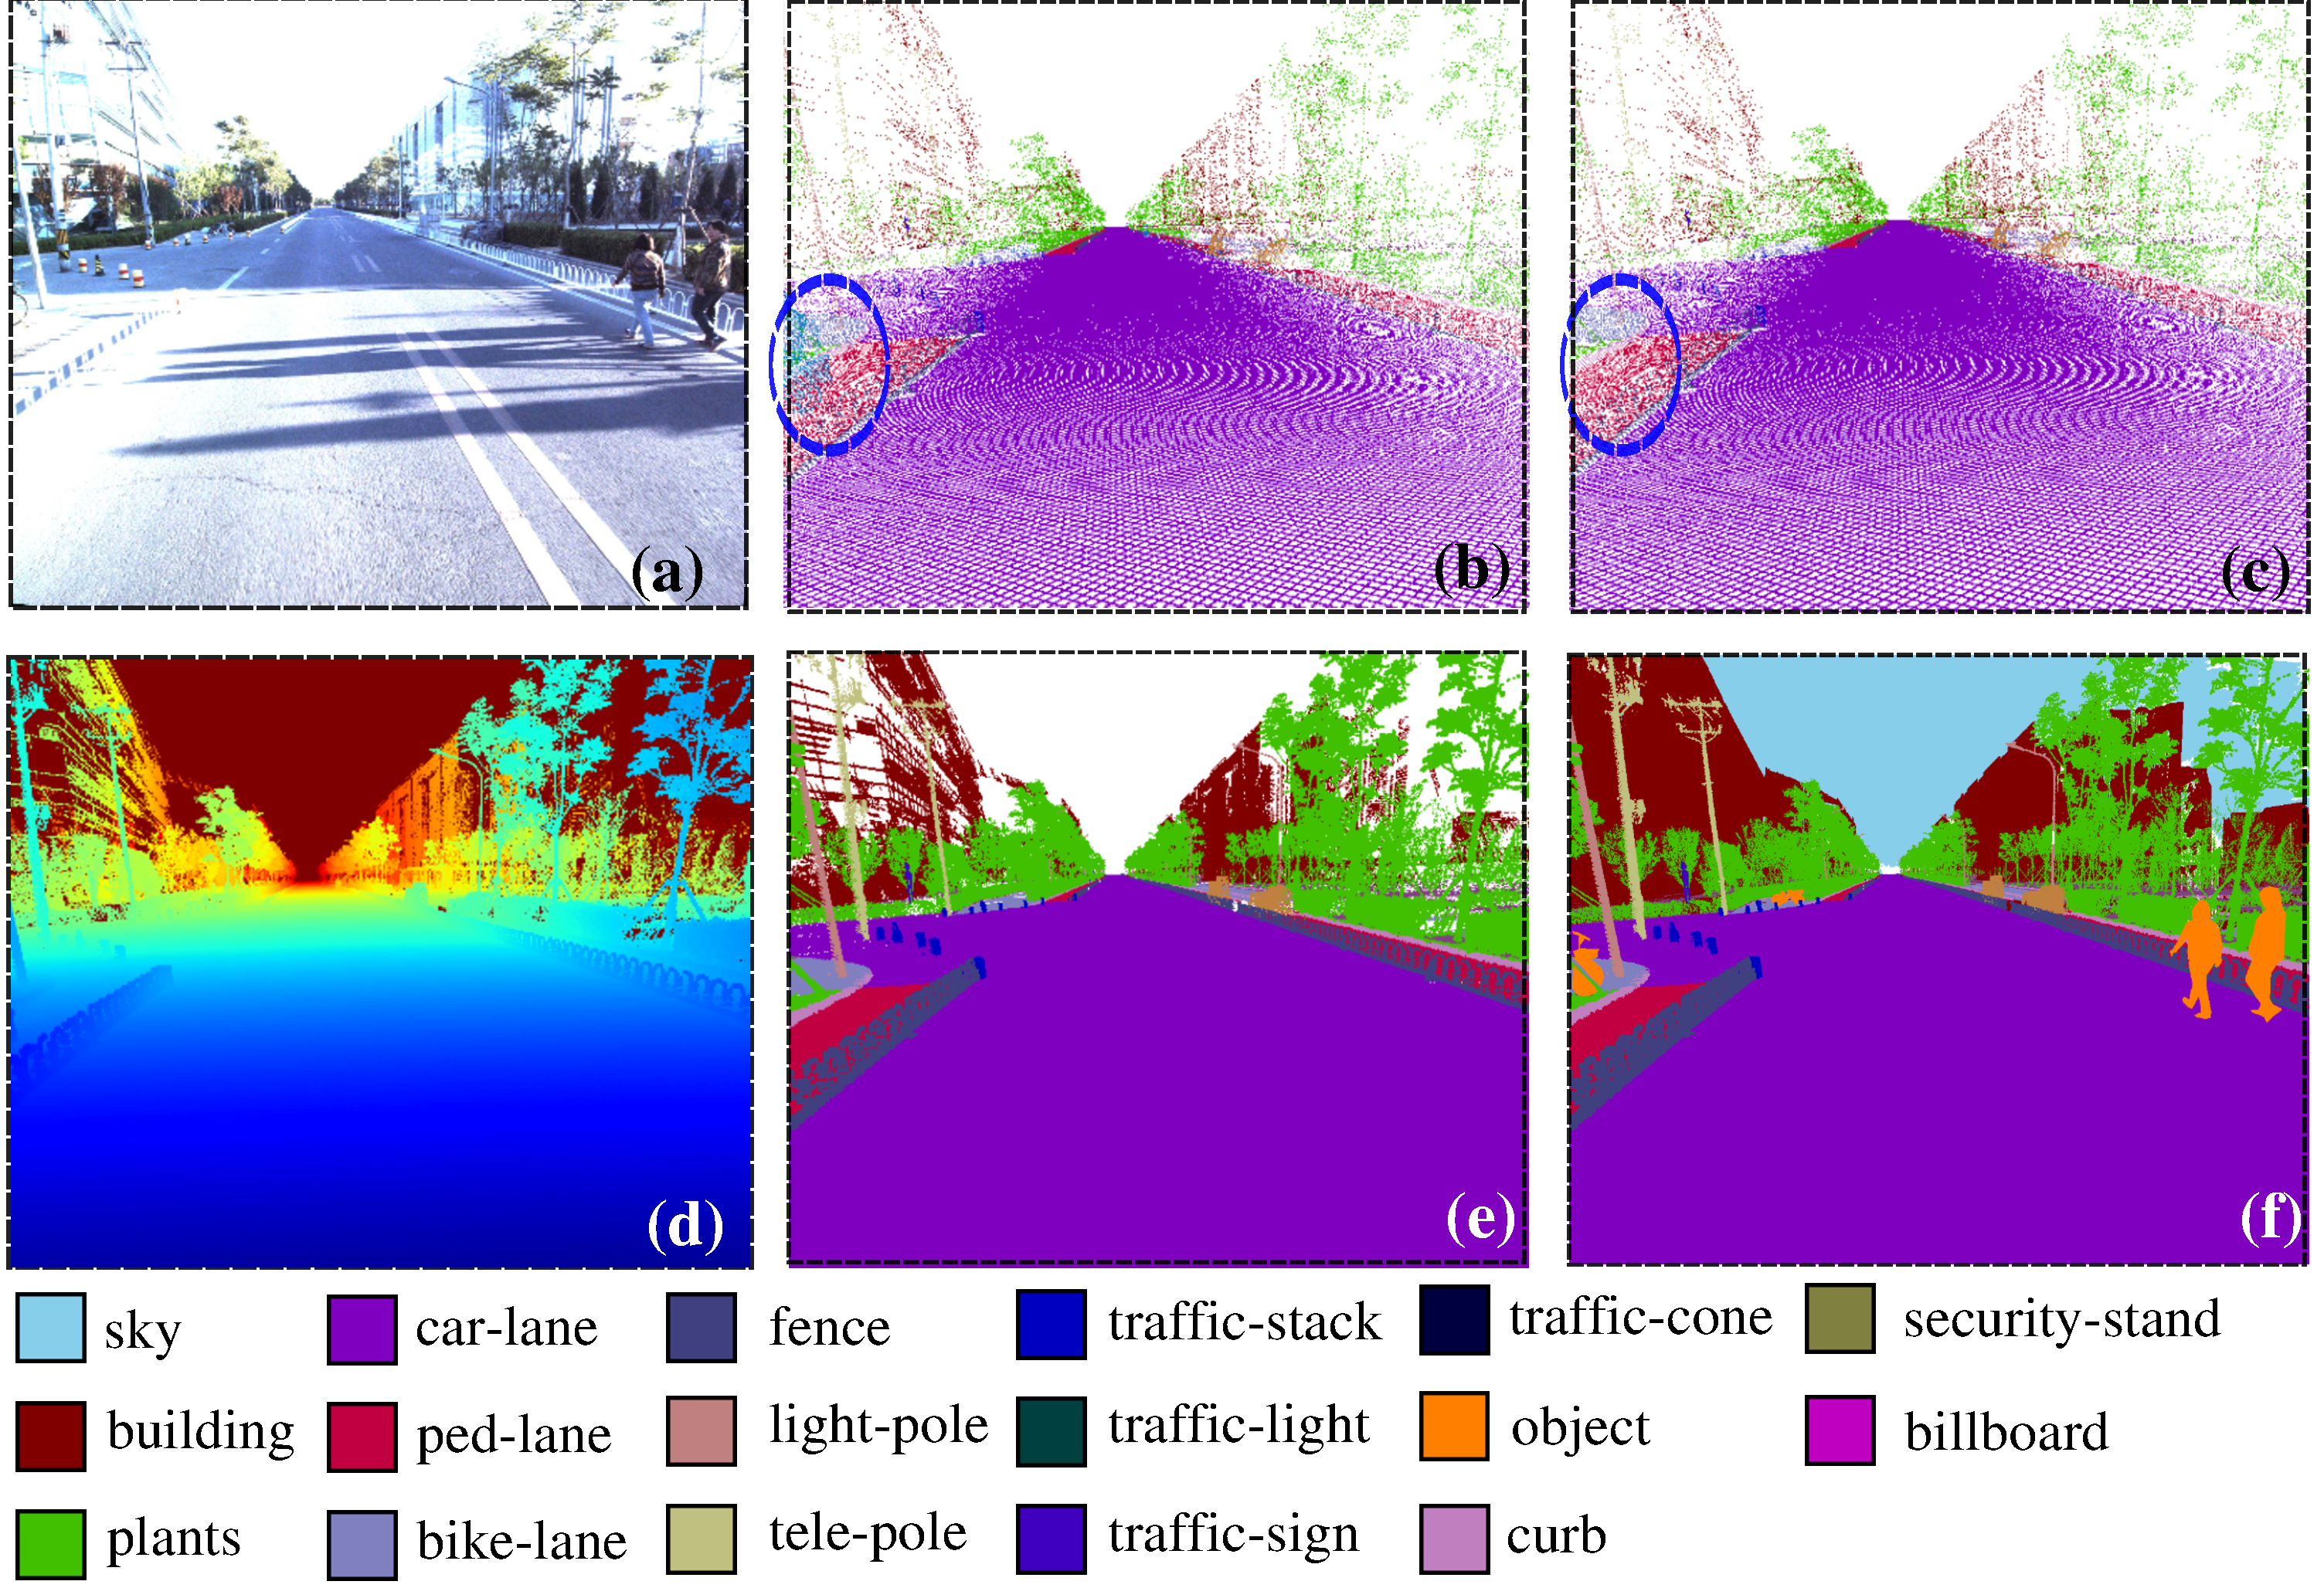
\includegraphics[width=\linewidth]{fig/dataset.pdf}
\vspace{-1.7\baselineskip}
\end{center}
	\caption{An example of our collected street-view dataset. (a) Image. (b) Rendered label map with 3D point cloud projection, with an inaccurate moving object (rider) circled in blue. (c)Rendered label map with 3D point cloud projection after points with low temporal consistency being removed. (d) $\&$ (e) Rendered depth map of background and rendered label map after class dependent splatting in 3D point clouds (\secref{sub:render}). (f) Merged label map with missing region in-painted, moving objects and sky.}
\label{fig:data}
\vspace{-1.3\baselineskip}
\end{figure}

% Undistortion of the image
%\paragraph{Label 3D map and videos.}
\textbf{2D and 3D labeling}
% talk about labelling in 3D
In order to have semantic labelling of each video frame, we handle static background, static objects (\eg parked vehicles that could be well recognized in point clouds), and moving objects separately.
Firstly, for static background, we directly perform labelling on the 3D point clouds $\hua{M}$ which are then projected to images, yielding labelled background for all the frames.
Specifically, we over-segment the point clouds into point clusters based on spatial distances and normal directions, and then label each cluster of points manually.
Second, for static objects in each round, we prune out the points of static background, and label the remaining points of the objects.
%Due to the fact that when object is static, \eg parked cars, the shape and location of captured points will be highly recognizable, whereas when the object is moving on the road, the points will be fuzzy, we ask labeller to label those can be well recognized as static objects.
Thirdly, after 3D-2D projection, only moving objects remain unlabeled. Here, we adopt an active labelling strategy, by first training an object segmentation model using a SOTA algorithm~\cite{WuSH16e}, and then refining the masks of moving objects manually.

As shown in \figref{fig:data}(c), the labels obtained from above three steps are still not perfect. There are some unlabeled pixels that could be caused by missing points or reflection. We handle such issue by using splatting techniques in computer graphics, which is to turn each point into a small squaure as discussed in \secref{sub:render} (\figref{fig:data}(e)). The results are futher refined to genereate the final labels (\figref{fig:data}(f)).
With such a strategy, we can greatly increase labelling efficiency and accuracy. For example, it could be very labor-intensive to label texture-rich regions like trees and poles, especially when occlusion happens.
We provided the labelled video in our supplementary materials for readers who are interested.

